\begin{figure}[t]
	\centering
	\definecolor{blue}{HTML}{1f77b4}%
\definecolor{red}{HTML}{d62728}%
\definecolor{green}{HTML}{2ca02c}%
\definecolor{yellow}{HTML}{fee23e}%
\definecolor{hidden}{HTML}{005b82}%
\definecolor{input}{HTML}{af5a50}%
\definecolor{ppu}{HTML}{7d966e}%
\definecolor{output}{HTML}{555555}%
\tikzset{silent/.style={cross out, draw, 
         minimum size=2*(3pt-\pgflinewidth), 
	 inner sep=0pt, outer sep=0pt, thick}}
\tikzset{input_synapse/.style={circle,minimum size=0.17cm,inner sep=0pt,fill=input}}%
\tikzset{recurrent0_synapse/.style={circle,minimum size=0.17cm,inner sep=0pt,fill=hidden}}%
\tikzset{recurrent1_synapse/.style={circle,minimum size=0.17cm,inner sep=0pt,fill=output}}%
\pgfmathdeclarerandomlist{MyRandomSynapses}{%
    {input_synapse}%
    {recurrent0_synapse}%
    {recurrent1_synapse}%
    {silent}%
}%
\tikzset{block/.style={font={\rmfamily\footnotesize},align=center}}%
\tikzset{box/.style={draw=black!90}}%
\tikzset{block label/.style={fill=white,font={\rmfamily\footnotesize},inner sep=0.05cm}}%
\tikzset{%
	neuron/.style = {%
		draw=black,%
		circle,%
		inner sep=0pt,%
		minimum width=0.3cm%
	},%
	driver/.style = {%
		minimum height=0.7cm,%
		draw=black,%
		regular polygon,%
		regular polygon sides=3,%
		shape border rotate=-90,%
		inner sep=0pt%
	},%
}%
%
\begin{tikzpicture}[
		x=1.7cm,
		y=1.7cm,
	    	anchor=center,
        ]
        \pgfdeclarelayer{background layer}
        \pgfsetlayers{background layer,main}
        % \draw[use as bounding box,inner sep=0pt,draw=none] (-0.1,0.0) rectangle ++(5.5,4.5);

	\begin{scope}
		\foreach \x in {0,1,...,7} {
			\pgfmathparse{100*(\x>3)}
			\colorlet{currentcolor}{output!\pgfmathresult!hidden}
			
			\node[neuron,currentcolor,thick,inner sep=1pt] (nrn \x) at (0.8 + \x*0.5,0.35) {\fontsize{8}{8}\selectfont $t_\x^k$};
			\draw[stealth-] (nrn \x.north) ++ (0.0,0.01) -- ++(0.0,1.85);
		}

		\foreach \y [evaluate=\y as \z using {int(\y + 4)}] in {0,1,...,3} {
			\node[driver,thick] (drv \y) at ($(nrn 0) + (-0.5,0.5 + \y*0.5)$) {};
			\draw (drv \y.east) -- ++(3.8,0.0);
			\draw[stealth-,input,thick] ($(drv \y.center) + (-0.11,0.10)$) -- ++(-0.25,0.0) node[anchor=east] {\fontsize{8}{8}\selectfont $s_\y^l$};

			\foreach \x in {0,1,...,7} {
				\pgfmathrandomitem{\RandomSynapse}{MyRandomSynapses}
				\draw (drv \y -| nrn \x) node[\RandomSynapse] {};
			}
		}

		% routing
		\foreach \x in {0,1,2,3} {
			\draw[hidden,thick] (nrn \x.south) -- ++(0.0,-0.1) coordinate (tmp) -- (tmp -| drv 0.west) -- ++(-0.14,0.0) coordinate (sammelpunkt);
		}
		
		\foreach \y in {0,1,...,3} {
			\draw[-stealth,hidden,thick] (sammelpunkt) -- ($(sammelpunkt |- drv \y) + (0.0,0.00)$) coordinate (tmp) -- (tmp -| drv \y.west);
		}
		
		\foreach \x in {4,5,6,7} {
			\draw[output,thick] (nrn \x.south) -- ++(0.0,-0.16) coordinate (tmp) -- (tmp -| drv 0.west) -- ++(-0.2,0.0) coordinate (sammelpunkt);
		}
		
		\foreach \y in {0,1,...,3} {
			\draw[-stealth,output,thick] (sammelpunkt) coordinate (tmp) -- ($(tmp |- drv \y) - (0.0,0.1)$) coordinate (tmp) -- (tmp -| drv \y.west);
		}

		% ppu
		\node[rectangle,thick,draw,ppu,rounded corners,inner sep=2pt,minimum width=6.5cm] (ppu) at ($(nrn 0) + (1.9,2.7)$) {\fontsize{8}{8}\selectfont PPU};
		\foreach \x in {0,1,...,7} {
			\draw[ppu,-stealth] (nrn \x.55) -- ++(55:0.12) coordinate (tmp) -- (tmp |- ppu.south) node[pos=0.85, fill=white, inner sep=1] {\fontsize{8}{8}\selectfont $\nu_\x$};
		}
	\end{scope}
\end{tikzpicture}

	\caption{%
		\textbf{The connectivity on BrainScaleS-2 is physically represented by two arrays of synapses.}
		The routing capabilities of BrainScaleS-2 are utilized such that both arrays can be treated as a larger virtual one.
		Input events $s_i^l$ enter this array together with recurrent events $t_i^k$ (blue and gray) from the left via synapse drivers (triangles).
		The latter forward the events to a whole row of synapses (circles).
		Each synapse locally filters incoming events and either transmits input events (red) or recurrent events (blue and gray) to its home neuron.
		Sparsity is implemented by silencing out synapses (black crosses).
		Homeostatic regulation is carried on by the on-chip \acrshort{ppu} by accessing neuronal firing rates $\nu_i$ to update synaptic weights in a row-wise parallel manner.
	}
	\label{fig:routing}
\end{figure}

\section{Hardware details} \label{sec:appendix_hardware}

The connectivity on BrainScaleS-2 is physically represented by two arrays of synapses, each with a set of $256\times 256$ synapses.
Input spikes $s_i^l$ enter these arrays from the left via synapse drivers and are forwarded to a whole row of synapses.
Each synapse within this row locally filters incoming events, weights them according to a \SI{6}{\bit} weight and eventually transmits them to its home neuron.
The neurons are arranged in an additional row below the array of synapses.
Emitted neuronal spikes are injected back into the array via a flexible on-chip spike router.

Within this work, we exploit the routing capabilities of the BrainScaleS-2 system to unify both synapse arrays to a virtual array of size $256\times 512$ (\cref{fig:routing}).
The event filtering within each synapse located between synapse driver $i$ and neuron $j$ is used to either transmit the input events of spike source $i$ or the recurrent events of the neuron $i$ or $i + 256$, respectively.
We map our networks by configuring a random set of on average $K^\mathrm{rec}$ synapses per column of synapses to transmit recurrent events.
In addition, on average $K^\mathrm{in}$ randomly chosen synapses relay the input spike trains.
All remaining synapses are configured to transmit no events.

On BrainScaleS-2, the effect of each synapse, i.\,e.\, excitatory or inhibitory, is determined by the synapse drivers and is therefore a row-wise property within the synapse array.
For our networks, we program \SI{20}{\percent} of the synapse drivers (randomly selected) to be inhibitory.

The homeostatic plasticity is implemented on-chip by drawing on both \glspl{ppu} \citep{friedmann_demonstrating_2017}.
To that end, the number of emitted spikes is accessed and loaded into the \gls{simd} vector units of the \glspl{ppu} for subsequent weight update calculations.
Each vector unit allows to update a half-row of synaptic weights ($128$) synapses in parallel.
Calculations are performed with a precision of \SI{8}{\bit} in a fractional-saturation arithmetic.
The random numbers required to implement stochastic weight updates are directly drawn in parallel on-chip via dedicated accelerators.

\begin{figure*}[ht]
	\centering
	\begin{tikzpicture}
		\node[anchor=north west,inner sep=0pt] (a) at (0,0) {\input{build/figures/v_leak.pgf}};
		\node[anchor=north west,inner sep=0pt] (b) at (0,-3.6) {\input{build/figures/v_thres.pgf}};
		\node[anchor=north west,inner sep=0pt] (c) at (4.4,0) {\input{build/figures/v_reset.pgf}};
		\node[anchor=north west,inner sep=0pt] (d) at (4.4,-3.6) {\input{build/figures/tau_m.pgf}};
		\node[anchor=north west,inner sep=0pt] (e) at (8.8,0) {\input{build/figures/tau_syn_exc.pgf}};
		\node[anchor=north west,inner sep=0pt] (f) at (8.8,-3.6) {\input{build/figures/tau_syn_inh.pgf}};
		\node[anchor=north west,inner sep=0pt] (g) at (13.2,0) {\input{build/figures/epsp_height.pgf}};
		\node[anchor=north west,inner sep=0pt] (h) at (13.2,-3.6) {\input{build/figures/ipsp_height.pgf}};
		\node at ($(a.north west) + (0.2,-0.2)$) {\textbf{A}};
		\node at ($(b.north west) + (0.2,-0.2)$) {\textbf{B}};
		\node at ($(c.north west) + (0.2,-0.2)$) {\textbf{C}};
		\node at ($(d.north west) + (0.2,-0.2)$) {\textbf{D}};
		\node at ($(e.north west) + (0.2,-0.2)$) {\textbf{E}};
		\node at ($(f.north west) + (0.2,-0.2)$) {\textbf{F}};
		\node at ($(g.north west) + (0.2,-0.2)$) {\textbf{G}};
		\node at ($(h.north west) + (0.2,-0.2)$) {\textbf{H}};
	\end{tikzpicture}
	\caption{%
		\textbf{Parameter distributions on the BrainScaleS-2 system.}
		Calibration routines allow to reduce the parameter spread between circuit instances by drawing on the configurability of BrainScaleS-2.
		The calibration targets for \textbf{(A)} the leak potential $u^\mathrm{leak}_i$ and \textbf{(B)} the threshold potential $u^\mathrm{thres}_i$ are chosen such that their distance is as high as possible.
		\textbf{(C)} The target for the reset potential is chosen slightly below $u^\mathrm{leak}_i$.
		\textbf{(D)} The excitatory synaptic time constants $\tau^\mathrm{s,exc}_i$ and \textbf{(E)} the inhibitory synaptic time constants $\tau^\mathrm{s,inh}_i$ are calibrated to coincide.
		\textbf{(F)} The membrane time constant $\tau^\mathrm{m}_i$ exceeds the synaptic time scales.
		Linear fits to measurements of the \acrshort{psp} height for various weight values $w_{ij}$ allow to estimate \textbf{(G)} the excitatory weight scaling factors $\gamma_i^\mathrm{exc}$ as well as \textbf{(H)} the inhibitory weight scaling factor $\gamma_i^\mathrm{inh}$.
	}
	\label{fig:parametrization}
\end{figure*}

\section{Calibration and parametrization \label{sec:parametrization}}

The fabrication induced device variations of the analog neuromorphic substrate are mitigated by calibration routines.
Here, we utilize bisection methods to adjust the neuro-synaptic parameters inferred from recorded traces to desired targets (\cref{fig:parametrization}).
Afterwards, the resulting \gls{lif} neuron parameters are measured and their mean as well as standard deviations are used for the parametrization of the equivalent software models.
To align the impact of a single spike on all downstream neurons on hard- and in software, we characterize the \gls{psp} height as a function of the configured weight value $w_{ij}$.
In more detail, we obtained the weight scaling factor $\gamma_i$ in \cref{eq:synapse} by fitting the ideal solution of \cref{eq:membrane}
\begin{align}
	u_i(t) = & \, u^\mathrm{leak} + \frac{\tau^\mathrm{m}\cdot\tau^\mathrm{s}\cdot \gamma_i w_{ij}}{C^\mathrm{m} (\tau^\mathrm{s} - \tau^\mathrm{m})} \Theta\left(t - t_j^0\right) \nonumber\\
	&\cdot\left[\exp{\left(-\frac{t-t_j^0}{\tau^\mathrm{s}}\right)} - \exp{\left(-\frac{t-t_j^0}{\tau^\mathrm{m}}\right)}\right] \, ,
	\label{eq:lif_solution}
\end{align}
to recordings of each neuron's membrane potential $u_i(t)$ in response to a single stimulating event $t_j^0$ relayed over a single synapse with weight $w_{ij}$.
To ensure stable fits, we fix all fit parameters to the calibration target values except for the leak potential $u^\mathrm{leak}$ and our estimate of $\gamma_i w_{ij}$ that we call $y$.
From the linear fit $y = \gamma_i w_{ij}$, we then obtain an estimate of $\gamma_i$ for excitatory and inhibitory weights respectively (\cref{fig:parametrization} G and H).
All estimated parameters are summarized in \cref{tab:parameters}.

\begin{table}[b]
	\centering
	\caption{%
		\textbf{Model parameters.}
		All parameters are given in the equivalent biological time domain.
		The errors indicate the standard deviation.
	}
	\label{tab:parameters}
	\footnotesize
\begin{ruledtabular}
	\begin{tabular}{llr}
		\textbf{Parameter} 			& \textbf{Symbol}		& \textbf{Value} \\
		\hline
		Membrane capacitance 			& $C^\mathrm{m}$		& \SI{2.4(2)}{\pico\farad} \\
		Threshold potential			& $u^\mathrm{thresh}$		& \SI{741(06)}{\milli\volt} \\
		Leak potential				& $u^\mathrm{leak}$		& \SI{458(43)}{\milli\volt} \\
		Reset potential				& $u^\mathrm{reset}$		& \SI{324(06)}{\milli\volt} \\
		Membrane time constant			& $\tau^\mathrm{m}$		& \SI{21.5(15)}{\milli\second} \\
		Excitatory synaptic time constant	& $\tau^\mathrm{s,exc}$		& \SI{5.3(3)}{\milli\second} \\
		Inhibitory synaptic time constant	& $\tau^\mathrm{s,inh}$		& \SI{5.4(2)}{\milli\second} \\
		Synaptic delay				& $\tau^\mathrm{d}$		& \SI{1.0(1)}{\milli\second} \\
		Refractory period			& $\tau^\mathrm{ref}$		& \SI{2.0}{\milli\second} \\
		Exciatotry weight scaling factor	& $\gamma^\mathrm{exc}$		& \SI{0.57(10)}{\nano\ampere} \\
		Inhibitory weight scaling factor	& $\gamma^\mathrm{inh}$		& \SI{0.67(10)}{\nano\ampere} \\
		\hline
		Recurrent synapses per neuron		& $K^\mathrm{rec}$		& \SI{100}{} \\
		Neurons					& $N$				& \SI{512}{} \\
		Input weight				& $w^\mathrm{in}$		& \SI{17}{} \\
		\hline
		Learning rate				& $\lambda$			& \SI{0.46875}{} \\
		Target rate				& $\nu^\ast$			& \SI{10}{\hertz} \\
		Update probability			& $p$				& \SI{2.3}{\percent} \\
		Number of updates			& $n$				& \SI{1000}{} \\
		\hline
		External rate				& $\nu^\mathrm{ext}$		& \SI{10}{\hertz} \\
		\hline
		Static experiment duration		& $T$				& \SI{100}{\second} \\
	\end{tabular}
\end{ruledtabular}

\end{table}

\begin{figure}[ht]
	\centering
	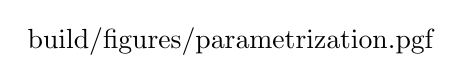
\begin{tikzpicture}
		\node[anchor=north west,inner sep=0pt] (a) at (0,0){\import{build/figures/}{parametrization.pgf}};
	\end{tikzpicture}
	\caption{%
		\textbf{Parametrization of the homeostatic regulation.}
		The homeostatic regulation is parametrized by the update acceptance probability $p$ as well as the learning rate $\lambda$.
		Shown is the variance of the firing rate of each neuron $\nu_i$ with respect to the target rate $\nu^\ast$, $\sqrt{\langle \left(\nu_i - \nu^\ast\right)^2\rangle}$, averaged over \num{100} experiments for an input rate of $h=\SI{0.6}{\kilo\hertz}$.
		The configuration used within the experiments presented in the main part is highlighted by the red star.
	}
	\label{fig:stability}
\end{figure}
\begin{figure*}[ht]
	\centering
	\begin{tikzpicture}
		\node[anchor=north west,inner sep=0pt] (a) at (0,0){\import{build/figures/}{phase_full_emul_60.pgf}};
		\node[anchor=north west,inner sep=0pt] (c) at (4.0,0) {\import{build/figures/}{phase_full_emul_80.pgf}};
		\node[anchor=north west,inner sep=0pt] (e) at (8.0,0.0) {\import{build/figures/}{phase_full_emul_100.pgf}};
		\node[anchor=north west,inner sep=0pt] (x) at (12.0,-0.1) {\import{build/figures/}{phase_full_emul_colorbar.pgf}};
		\node[anchor=north west,inner sep=0pt] (g) at (13.6,0.0) {\import{build/figures/}{phase_full_emul_cross.pgf}};

		\node[anchor=north west,inner sep=0pt] (b) at (0.0,-4.4) {\import{build/figures/}{phase_full_sim_60.pgf}};
		\node[anchor=north west,inner sep=0pt] (d) at (4.0,-4.4) {\import{build/figures/}{phase_full_sim_80.pgf}};
		\node[anchor=north west,inner sep=0pt] (f) at (8.0,-4.4) {\import{build/figures/}{phase_full_sim_100.pgf}};
		\node[anchor=north west,inner sep=0pt] (y) at (12.0,-4.5) {\import{build/figures/}{phase_full_sim_colorbar.pgf}};
		\node[anchor=north west,inner sep=0pt] (h) at (13.6,-4.4) {\import{build/figures/}{phase_full_sim_cross.pgf}};

		\node at ($(a.north west) + (0.2,-0.2)$) {\textbf{A}};
		\node at ($(b.north west) + (0.2,-0.2)$) {\textbf{B}};
		\node at ($(g.north west) + (0.2,-0.2)$) {\textbf{C}};
		\node at ($(h.north west) + (0.2,-0.2)$) {\textbf{D}};
		\node[draw,fit=(b) (h)] (box_simulation) {};
	\end{tikzpicture}
	\caption{%
		\textbf{Phase diagrams of networks with homogeneous and static weights.}
		\textbf{(A)} The firing rates $\nu$ for three exemplary input rates $h$ are comparable between hardware \textbf{(A)} and software \textbf{(B)} implementations.
		However, there is a small shift of the transitions from high firing rates $\nu$ to intermediate firing rates between both.
		For each value of the configured inhibitory weight $w^\mathrm{inh}$, the firing rate is closest to \SI{10}{\hertz} for a coinciding excitatory weight $w^\mathrm{exc}_\mathrm{cross}$ for both, emulation \textbf{(C)} as well as simulation \textbf{(D)}.
	}
	\label{fig:phase_full}
\end{figure*}

\section{Parametrization of the homeostatic regulation \label{sec:hom_parametrization}}

The homeostatic regulation as given by \cref{eq:rule} comes with two independent parameters: the learning rate $\lambda$ as well as the update acceptance probability $p$.
We obtained optimal parameters by performing a grid search for $h = \SI{0.6}{\kilo\hertz}$ and assessing the variance of the firing rate of all neurons $\nu_i$ with respect to the target rate $\nu^\ast$, i.\,e\,. $\sqrt{\langle \left(\nu_i - \nu^\ast\right)^2\rangle}$.
For a broad range of parameters, most of the \gls{lif} neurons emit spikes at a rate resembling the target rate (\cref{fig:stability}).
Only for low values of $\lambda$ and high values of $p$, the firing rate systematically deviates due to the integer arithmetic used for weight update calculations on the neuromorphic system.

Most notably, we also used the determined optimal parameters within our software simulations.
This pursued strategy renders extensive parameter sweeps in software superfluous and moreover showcases the benefits of the accelerated analog emulation of neuro-synaptic dynamics due to the referenced efficiency in terms of speed and power consumption.

\begin{figure*}[ht]
	\centering
	\begin{tikzpicture}
		\node[anchor=north west,inner sep=0pt] (a) at (0,0){\import{build/figures/}{phase_rate.pgf}};
		\node[anchor=north west,inner sep=0pt] (b) at (4.5,0) {\import{build/figures/}{phase_taus.pgf}};
		\node[anchor=north west,inner sep=0pt] (c) at (9.0,0.0) {\import{build/figures/}{phase_fano.pgf}};
		\node[anchor=north west,inner sep=0pt] (d) at (13.5,0.0) {\import{build/figures/}{phase_cv.pgf}};

		\node[anchor=north west,inner sep=0pt] (e) at (0.0,-4.2) {\import{build/figures/}{phase_activity_distribution_0.pgf}};
		\node[anchor=north west,inner sep=0pt] (f) at (4.5,-4.2) {\import{build/figures/}{phase_activity_distribution_1.pgf}};
		\node[anchor=north west,inner sep=0pt] (g) at (9.0,-4.2) {\import{build/figures/}{phase_activity_distribution_2.pgf}};
		\node[anchor=north west,inner sep=0pt] (h) at (13.5,-4.2) {\import{build/figures/}{phase_activity_distribution_3.pgf}};

		\node[anchor=north west,inner sep=0pt] (i) at (0,-8.4){\import{build/figures/}{phase_raster_0.pgf}};
		\node[anchor=north west,inner sep=0pt] (j) at (4.5,-8.4){\import{build/figures/}{phase_raster_1.pgf}};
		\node[anchor=north west,inner sep=0pt] (k) at (9.0,-8.4){\import{build/figures/}{phase_raster_2.pgf}};
		\node[anchor=north west,inner sep=0pt] (l) at (13.5,-8.4){\import{build/figures/}{phase_raster_3.pgf}};
		\node at ($(a.north west) + (0.2,-0.2)$) {\textbf{A}};
		\node at ($(b.north west) + (0.2,-0.2)$) {\textbf{B}};
		\node at ($(c.north west) + (0.2,-0.2)$) {\textbf{C}};
		\node at ($(d.north west) + (0.2,-0.2)$) {\textbf{D}};
		\node at ($(e.north west) + (0.2,-0.2)$) {\textbf{E}};
		\node at ($(i.north west) + (0.2,-0.2)$) {\textbf{F}};
	\end{tikzpicture}
	\caption{%
		\textbf{Dynamics of networks with homogeneous and static weights.}
		\textbf{(A)} The transitions from high firing rates $\nu$ to intermediate firing rates occurs in the vicinity of $g\approx 1$ for decreasing $h$.
		\textbf{(B)} The autocorrelation time $\tau_\mathrm{AC}$ and \textbf{(C)} the Fano factor are estimated based on the population activity obtained with a bin size of \SI{5}{\milli\second} and show peaks around the finite-size transition.
		\textbf{(D)} Average Coefficient of variation of single neuron inter-spike intervals suggests regular spiking for small $g$ and irregular spiking for large $g$.
		\textbf{(E)} Distributions of population rates shown in (A) for slices of different $g$ show the transition from regular firing at high rates to irregular firing at low rates.
		\textbf{(F)} Example snapshots of spike rater plots and population rate for $h=\SI{0.7}{\kilo\hertz}$ for different $g$.
	}
	\label{fig:phase}
\end{figure*}


\section{Phase diagrams of networks with homogeneous and static weights \label{sec:phase_diagrams}}

To understand why we can observe fluctuating or bistable dynamics in networks with homeostatically regulated weights despite apparent excitation dominance (cf.\ \cref{fig:chip} and \cref{fig:time_scale}), we study here the phase diagram of comparable networks with homogeneous and static weights.
Due to small fluctuations in the transition point for different realizations of small networks, we focus on a single network realization and split the measurement into \num{200} blocks of length $\SI{30}{\second}$.
To ensure spiking activity even for low input strengths $h$, we initially increased $h$ for \SI{5}{\second} and subsequently let the networks equilibrate for another \SI{5}{\second}.

We first perform a full sweep over the $w_\mathrm{exc}-w_\mathrm{inh}$ plane on both the BrainScaleS-2 and a corresponding software simulations for three exemplary input strengths (\cref{fig:phase_full} A and B).
While the overall trend of the firing rates in emulation and simulation is quite comparable, the transition from low to high firing rates is clearly shifted.
We attribute these remaining differences to (i) the fact that our simulations do not capture correlations in the variability of parameters, but instead implement uncorrelated Gaussian noise, and (ii) to additional saturation effects within the analog circuits of BrainScaleS-2.

When we consider as a proxy for the transition between high-firing and low-firing phase the line where $\nu\approx 10$, we notice that this transition occurs for $w^\mathrm{exc} \approx \left(w^\mathrm{inh} + o\right)/s$ with $o>0$ an $h$-dependent offset (\cref{fig:phase_full} C and D).
Hence, this transition does not occur for a fixed inhibition-excitation ratio, $g=w^\mathrm{inh}/w^\mathrm{exc} \approx s - o/w^\mathrm{exc}$.
Instead, $g$ depends non-trivially on the excitatory coupling as well as on the parameters $s$ and $o$, which further depend on the input rate $h$ and the specific choice of input coupling (see \cref{sec:methods}).

When we now interpret our symmetric homeostatic rule to only allow identical couplings $w_\mathrm{exc}=w_\mathrm{inh}$ (\cref{fig:phase_full} C and D, black dashed line), then homeostatic plasticity should adjust the weights to the intersection between the transition lines and the unit line.
While this is strongly simplified, it approximately recovers the range of resulting mean weights that we find for the homeostatically-regulated neuromorphic chip (\cref{fig:chip}) and simulations (see Supplemental Material).

To characterize the dynamical phases of high- and low-firing rates, we focus on the special cut plane of $w^\mathrm{exc}=w^\mathrm{in}=17$ on the BrainScaleS-2 system.
We record the mean neuron firing rate, the integrated autocorrelation time, the network Fano factor, as well as the coefficient of variation (CV) of inter-spike intervals as a function of the inhibition dominance, $g=w^\mathrm{inh}/w^\mathrm{exc}$.
%
The integrated autocorrelation time is estimated from integrating the autocorrelation function $C(t^\prime)$, cf.\, \cref{eq:correlation}.
We follow the common convention~\cite{grotendorst_statistical_2002} to define $\tau_\mathrm{int}=\Delta t[\frac{1}{2}+\sum_{l=1}^{l_\mathrm{max}} C(l)]$, where $l_\mathrm{max}$ is self-consistently obtained as the first $l$ for which $l > 6\,\tau_\mathrm{int}(l)$.
This reliably estimates the scale of temporal correlations for fully sampled systems and did not become unstable due to the typical oscillations in the autocorrelation function observed for networks of \gls{lif} neurons.
Since the communication bottleneck of the hardware constrained long samples for high firing rates, we partitioned each recording into $L=\num{200}$ chunks of size $T=\SI{30}{\second}$ and estimated for each chunk the moments as averages, i.e., $\overline{\nu(t)}_l=\frac{1}{T}\sum_t \nu(t)$ and $\overline{\nu(t)\nu(t+t^\prime)}_l=\frac{1}{T}\sum_t \nu(t)\nu(t+t^\prime)$.
To avoid finite-data biases~\cite{marriott_bias_1954}, we then first obtained the best estimates of the mean $\overline{\nu(t)}=\frac{1}{L}\sum_l\overline{\nu(t)}_l$ and analogously of the correlation term, to then estimate the covariance as $\text{Cov}[\nu(t+t^\prime)\nu(t)]=\overline{\nu(t)\nu(t+t^\prime)} - \overline{\nu(t)}^2$.
%
Similarly, we estimate the network Fano factor on the population rate as the ratio between variance and mean, i.e., $F=(\overline{\nu^2(t)}-\overline{\nu(t)}^2)/\overline{\nu(t)}$, and the CV as average across neurons, i.e. $\text{CV}=\frac{1}{N}\sum_i \sqrt{\overline{\delta t^2}_i-\overline{\delta t}^2_i}/\overline{\delta t}_i$ with inter-spike-intervals $\delta t_i^j$ of neuron $i$.

We find that for the considered setup with an \gls{ei} input layer, the transition from high firing rates to low firing rates is reminiscent of a regular-to-irregular transition (\cref{fig:phase}A).
For the special choice $w^\mathrm{exc}=w^\mathrm{in}$, the transition occurs at $g\approx 1$ for $h\to0$, where the dynamic phase in the inhibition-dominated regime appears absorbing despite non-vanishing input due to the small system size.
In the vicinity of the $h$-dependent transition, we observe peaks in the autocorrelation time (\cref{fig:phase}B), which we expect to vanish due to the absorbing state in the limit of $h\to 0$ and $N\to\infty$~\cite{zierenberg_notitle_nodate}.
We find that the network Fano factor, estimated from the population activity with $\Delta t = \SI{5}{\milli\second}$ (\cref{fig:phase}C), is zero in the regular phase and low in the irregular phase, separated again by a peak that shifts towards $g=1$ with decreasing $h$ and becomes narrower.
Last, we observe the average coefficient of variation of single-neuron inter-spike intervals to change from $\text{CV}\approx 0$ for $g<1$, indicating regular spiking, to $\text{CV}\approx 1$ above the transition, indicating irregular spiking (\cref{fig:phase}D).

To illustrate the dynamic phases of regular and irregular activity, we show distributions of population rates (\cref{fig:phase}E) as well as spike raster plots and the time evolution of the population rate (\cref{fig:phase}F).
For $g=17/17=1$ we find all $h$ in a stable active state.
For $g=20/17\approx 1.2$ $h=\SI{0.3}{kHz}$ is already in the quiescent state, while $h=\SI{0.5}{kHz}$ shows strong variance between high rate and low rates that hinder estimation of autocorrelation times, but all other $h$ remain mostly in the stable active state.
For $g=26/17\approx 1.5$, we observe highest autocorrelations for $h=\SI{0.7}{kHz}$ due to strong fluctuation-driven excursions into the high-firing rate regime.
Further increasing $g$ also causes the other $h$ to fall into low-firing-rate states, where for small $h$ the state appears absorbing with practically no population activity following upon the few external perturbations.
Note that single points of the phase diagrams cannot be directly compared to the results after homeostatic regulation, which results in heterogeneous weight distributions (cf. \cref{fig:chip}E), because we here fix $w^\mathrm{exc}=w^\mathrm{in}$.

\begin{figure}[ht]
	\centering
	\begin{tikzpicture}
		\node[anchor=north west,inner sep=0pt] at (0,0){\import{build/figures/}{avalanche_distribution.pgf}};
	\end{tikzpicture}
	\caption{%
        \textbf{Tail of avalanche-size distribution from homeostatically regulated neuromorphic networks can be explained by the timescales of a \gls{hmm}.}
        Empirical avalanche-size distributions for different $h$ in a log-binned representation show now power-law shape.
        In contrast, the cutoff scale of their tails coincide with estimates from corresponding \gls{hmm}.
	}
	\label{fig:avalanches}
\end{figure}

\section{Avalanche analysis reveals} \label{sec:avalanches}
To verify that the autocorrelations we observe are not a result of close-to-critical fluctuations, we investigate the distribution of avalanche sizes.
For (self-organized) critical systems, one would expect avalanche sizes $s$ to be scale free~\cite{bak_self-organized_1988, pruessner_self-organised_2012}, i.e., an avalanche-size distribution $p(s)$ that can be described by a power law.

Here, we follow the convention to estimate avalanches from a time-discrete firing rate $\nu(t)$~\cite{beggs_neuronal_2003, zeraati_self-organization_2021}.
To constrain the temporal bin size to causal activity propagation, we estimate the spike delay from the solution of the \gls{lif} equation, \cref{eq:lif_solution}.
More specifically, the peak of the \gls{epsp} is an estimate of the maximal time until a certain spike can causally induce a threshold crossing.
We obtain the peak time of the \gls{epsp} from the condition $du / dt = 0$ in \cref{eq:lif_solution}, which together with the spike delay yields
\begin{equation}
	\tau^\mathrm{tot} = \tau^\mathrm{d} + \frac{\tau^\mathrm{m}\tau^\mathrm{s} \log{\left(\frac{\tau^\mathrm{m}}{\tau^\mathrm{s}}\right)}}{\tau^\mathrm{m} - \tau^\mathrm{s}} \, .
\end{equation}
Since $\tau^\mathrm{tot}$ sets an upper estimate of the causal delay, we here set the bin size for avalanche detection to $\Delta t = \tau^\mathrm{tot} / 2 = \SI{5}{\milli\second}$, in agreement with our previous time discretization.
An avalanche is then defined as the number of spikes in consecutive non-empty bins in $\nu(t)$, for which we measured $L=\num{200}$ chunks of size $T=\SI{100}{\second}$.

The resulting avalanche-size distributions do not show power-law behavior as expected close to a non-equilibrium phase transition (\cref{fig:avalanches}, data points).
In fact, we can compare the tails of the avalanche-size distribution with expectations from a 2-state \gls{hmm} (dashed lines).
For this, we assume that for the \gls{hmm} the state durations are be exponentially distributed (which we confirmed for low $h$, not shown).
Introducing a life-time $T_+$ and a conditional average rate $\nu_{+}$ for the high-firing state, we can approximate large avalanches sizes as $s=\nu_{+}T_+$ with $p(s) \propto p(T_+=s/\nu_+)$.
Since we do not have an unbiased estimate of the fraction of avalanches in the low-firing rate, we constrain the amplitude to align the tails of corresponding distributions.
The visual match between distribution tails indicate that in all cases we observe an exponential decay with a cutoff scale consistent with that of an \gls{hmm}.
We thus conclude that the empirical avalanche-size distributions show no sign of scale-free avalanches.

\section{Simulation of mean-field model} \label{sec:appendix_meanfield}

To simulate the time evolution of the mean-field model, one needs special care to avoid negative densities from numerical imprecisions that would render the multiplicative noise imaginary~\cite{dornic_integration_2005}.
In short, the steps involve first evaluating an exact solution of the noise and linear terms and then an Euler integration of the remaining quadratic term.
The precise mean-field equation we solve is
\begin{align}
    \dot{\rho}(t) = &h - \left(\tau_\mathrm{MF}-\alpha +h[1+\beta]\right)\rho(t)+ \sigma\sqrt{\rho(t)/N}\eta(t)\nonumber\\
    &-b\rho^2(t) \, .
\end{align}
This equation is decomposed into the linear term plus noise (first line), for which one can obtain an analytical solution, and the higher-order term (second line), which can be trivially integrated.

For the square-root noise plus linear term, i.e., $\dot{\rho}(t)=h+a\rho +\tilde{\sigma}\sqrt{\rho}\eta$, starting from $\rho(t)=\rho_0$ one knows the solution of the Fokker Planck equation for time $t+\Delta t$ is~\cite{feller_two_1951}
\begin{align}
    P(\rho,t+\Delta t) = \lambda e^{\lambda\left(\rho_0\omega+\rho\right)}\left[\frac{\rho}{\rho_0\omega}\right]^{\mu/2} I_\mu\left(2\lambda\sqrt{\rho_0\rho\omega}\right),
\end{align}
where $I_\mu$ is the modified Bessel function of order $\mu$, $\omega=e^{a\Delta t}$, $\lambda=2a/\sigma^2\left(\omega-1\right)$, and $\mu=-1+2h/\sigma^2$.
Using a Taylor-series expansion of the Bessel function, it was shown in Ref.~\cite{dornic_integration_2005} that rewriting $P(\rho,t+\Delta t)$ implies the density after $\Delta t$ can be simply drawn from the mixture
\begin{align}\label{eq:step1}
    \rho^\ast = \text{Gamma}\left[\mu + 1 + \text{Poisson}\left[\lambda\rho_0\omega\right]\right]/\lambda.
\end{align}

We thus evolve $\rho(t)$ in discrete time steps $\Delta t$ in two steps~\cite{dornic_integration_2005}:
First, we generate from $\rho_0=\rho(t)$ the stochastic solution $\rho^\ast$ using \cref{eq:step1}.
Second, we integrate the remaining term as $\rho(t+\Delta t)=\rho^\ast/(1+\rho^\ast b \Delta t)$.

For the example we show in \cref{fig:theory}, we used $\Delta t=10^{-7}$, $\tau=10$, $\alpha=19$, $\beta=10$, $b=12$, $\sigma=40$, and $N=512$. For further details we refer to the available code~\cite{noauthor_benjamincramerneuromorphic-bistability_nodate}.
